\section{Question-type based QA system} \label{approach2}

We now present a QA system which is a combination of several modules, each built to handle a specific question type. The reason we believe that such a system would be effective is because of that, in this case, the nuances of each of the question types can be appropriately captured in the modules and the modifications to one module to address its corresponding inadequacies will not affect the performance of any other. 
We build this system for the BioASQ dataset, primarily because of the unique challenges that the BioASQ dataset which call for a modularized system. 

In the sections that follow, we shall present the modules for handling the question types: yes/no, factoid/list and summary type. In addition to addressing each question type specifically, we also cater to different answer types: exact and ideal. Exact answers represent the subset of the BioASQ task where the responses are not structured paragraphs, but instead either a single entity (\textit{yes/no} types) or a combination of named entities (\textit{factoid} or \textit{list} types) that compose the correct reply to the given query. The main idea refers to evaluating if a response is able to capture the most important components of an answer. For factoid or list types of questions, we must return a list of the most likely entities to compose the answer. The main difference between them is that ground truth for \textit{factoid} questions is composed of only one correct answer and the evaluation method is Mean Reciprocal Rank (MRR). However, the ground truth for \textit{list} is an actual list of correct answers with varying length, which uses F-measure as an evaluation metric. The BioASQ submission format allows everyone to submit 5 ranked answers for \textit{factoid} and 1 to 10 answers for \textit{list}. For \textit{yes/no} questions, the ground truth is simply the yes or no label, using F-measure as an evaluation metric.

\subsection{Yes/No Type Questions}


Although yes/no questions require a simple binary response, calculating yes/no responses for a BioASQ question can be challenging for the following reasons: 
\begin{enumerate}
    \item There is an inherent class-bias towards the questions answered by \texttt{yes} in the dataset
    \item The dataset is quite small for training a complex semantic classifier
    \item An effective model must perform  reasoning and inference using the limited information it has available, which is extremely difficult even for non-expert humans
\end{enumerate}


Due to the nature of the question type, these questions can not be simply classified by using word-level features. Learning the semantic relationship between the question and the sentences in the documents is quite elemental to solving this task. Hence, we adopt a Natural Language Inference (NLI)-based system that learns if the assertions made by the questions are true in the context of the documents. Since most of the well-performing NLI models today are neural models, one of the biggest obstacles for this approach would be to be able to augment the BioASQ dataset with existing NLI datasets in a meaningful fashion. 

\subsubsection{Hypotheses}

Two key challenges that we faced in building a yes/no classifier were - a) the shallow bag-of-words models cannot capture the semantic relationships that are required to answer a yes/no question, and b) the are inadequate NLI datasets for biomedical domain, and the large NLI datasets that are available employ significantly different vocabularies using Global Vectors for Word Representation (GloVe) embeddings. \\ 

In light of these challenges, we devise the following hypotheses for the yes/no type questions:

\begin{enumerate}
    \item Yes/No questions can be modeled as an NLI task by creating assertions from the questions and assessing textual entailment among the snippets/documents
    \item We can enable transfer learning for BioASQ dataset using pre-trained neural models that use GloVe embeddings by projecting bio embeddings as well as GloVe embeddings to a common space
\end{enumerate}

To test these hypothesis, we train a Recognizing Textual Entailment (RTE) model for a standard NLI dataset, and fine-tune it for the BioASQ dataset using our proposed word-embedding projection technique. We then generate assertions from questions and evaluate the entailment or contradiction of these assertions using the RTE model. Using these entailment scores for all the sentences in the snippets or documents, we heuristically evaluate the answer to the yes/no question. 

\begin{figure}[t]
    \centering
    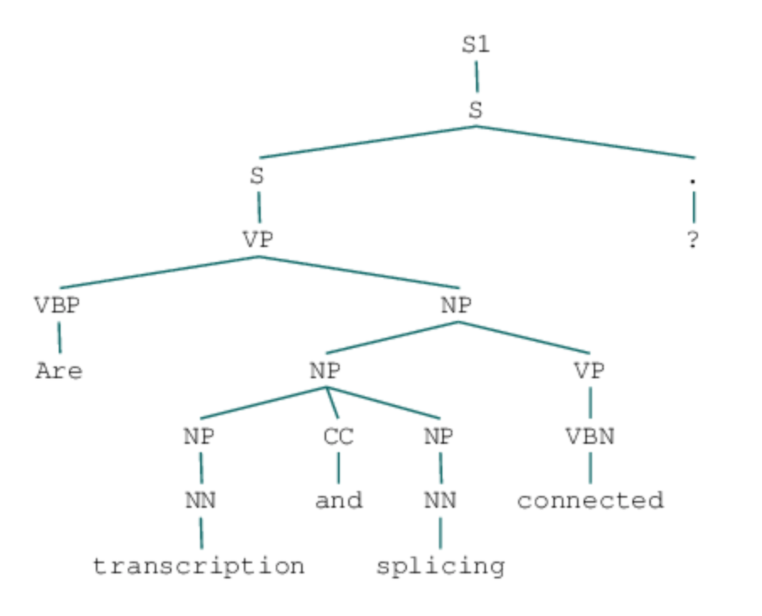
\includegraphics[scale=0.5]{images/question_parse.png}
    \caption{The parse tree of an example question as generated by the BLLIP parser}
    \label{fig:parse_tree}
\end{figure}

\subsubsection{Assertion Extraction}

The first step towards answering the question is to identify the assertions made by the question. For this, we use a statistical natural language parser to identify the syntactical structure in the question. We, then, heuristically generate assertions from the questions.\\

Consider the following example question:

\textit{Is the monoclonal antibody Trastuzumab (Herceptin) of potential use in the treatment of prostate cancer?}

Upon parsing of this question, we have the phase constituents of the question. As shown in the example in Figure \ref{fig:parse_tree}, almost all yes/no questions have a standard format that begins with an auxiliary verb followed by a noun phrase. In this example, we can toggle the question word with the first noun phrase to generate the assertion:

\textit{The monoclonal antibody Trastuzumab (Herceptin) is of potential use in the treatment of prostate cancer.}

In a similar manner, we then create positive assertions for all \textit{yes/no} questions as depicted in Table \ref{tab:assertion_examples}. As a simple extension to this, we can also create negative assertions by using \textit{not} along with the auxiliary verbs.

\begin{table*}[t!]
    \centering
    \begin{tabular}{r l} \hline
        Question & Assertion \\ \hline
    \textit{Is} the protein Papilin secreted? & The protein Papilin \textit{is} secreted \\
    \textit{Are} long non coding RNAs spliced? & 
    long non coding RNAs \textit{are} spliced \\
    \textit{Are} transcription and splicing connected? &
    Transcription and splicing \textit{are} connected. \\
    \textit{Is} RANKL secreted from the cells? &
    RANKL \textit{is} secreted from the cells. \\
    \textit{Does} metformin interfere thyroxine absorption? & 
    Metformin \textit{does} interfere thyroxine absorption. \\
    \textit{Has} Denosumab (Prolia) been approved by FDA? &
    Denosumab (Prolia) \textit{has} been approved by FDA. \\
    % \textit{Is} Alu hypomethylation associated with breast cancer? & 
    % Alu hypomethylation \textit{is} associated with breast cancer  \\
    \hline
   \end{tabular}
    \caption{Assertion generation for some questions from training set in BioASQ Phase 6b by heuristic-based rearrangement of the auxiliary verb the questions starts with.}    \label{tab:assertion_examples}
\end{table*}

\subsubsection{Recognizing Textual Entailment}

The primary goal of our NLI module is to infer if any of the sentences among the answer snippets entails or contradicts the assertion posed by the question. We segment the answer snippets for each question to produce a set of assertion-sentence pairs. To then evaluate if these assertions can be inferred or refuted from the sentences, we build a Recognizing Textual Entailment (RTE) model using the \textit{InferSent} model \cite{Infersent}, which computes sentence embeddings for every sentence and has been shown to work well on NLI tasks. In training \textit{InferSent}, we experience two major challenges:

\begin{enumerate}
    \item The number of assertion-sentence pairs in BioASQ is too few to train the textual entailment model effectively.
    \item The models that are pre-trained on SNLI \cite{snli}
    datasets use GLOVE \cite{glove} embeddings that cannot be used for biomedical corpora which have quite different characteristics and vocabulary compared to the corpora that GLOVE was trained on.
\end{enumerate}

However, we have pre-trained embeddings available that were trained on PubMed and PMC texts along with Wikipedia articles \cite{biomed_embed}. To leverage these embeddings, we implement an embedding-transformation methodology to projecting the PubMed embeddings to GLOVE embedding space and then fine tune the pre-trained \textit{InferSent} on the BioASQ dataset for textual entailment. The hypothesis is that, since both the embeddings had a significant fraction of documents in common (Wikipedia corpus), by transforming the embeddings from one space to another, the sentence embeddings from the model would still represent a lot of the semantic features of the input sentences that can subsequently used for classifying textual entailment. For this task, we explore both linear and non-linear methods of embedding transformation.

\subsubsection*{Linear transformation}

While simple, a linear projection of embeddings from one space to another has shown to be quite effective for a lot of multi-domain tasks. By imposing an orthogonality constraint on the project matrix, we model this problem as an orthogonal Procrustes problem: \\

Let $d_p$ and $d_g$ be the embedding dimensions of PubMed embeddings and GLOVE embeddings respectively.
If $E_p$ and $E_g$ are the matrices of PubMed embeddings ($N \times d_p$) and their corresponding GLOVE embeddings ($N \times d_g$) for the words that both the embeddings have in common ($N$), the projection matrix ($d_g \times d_p$) can be computed as,
\begin{align*}
    W^* &= \argmin_W \lVert  W E_p^{\intercal} - E_g^{\intercal} \rVert
\end{align*}
subject to the constraint that $W$ is orthogonal.

The solution to this optimization problem is given by using the singular value decomposition of $E_g^{\intercal} E_p$, i.e.
\begin{align*}
    W^* &= UV^{\intercal}, \\
    \text{where, } \\
    E_g^{\intercal} E_p &= U \Sigma V^{\intercal}
\end{align*}

With this simple linear transformation, we then compute the transformed embeddings for all the words in the PubMed embeddings that are not present in the GLOVE embeddings. 

\subsubsection*{Non-Linear Transformation}

We also explore a non-linear transformation using a feed-forward neural network, the objective is to learn function $f$ such that,
\begin{align*}
    f(e_p; \theta) = e_g
\end{align*}
where, $e_p$ and $e_g$ are PubMed and GLOVE embeddings respectively. We model $f$ using a deep neural network with parameters $\theta$, and train using the common words in both the embeddings. The effectiveness of this training is a result of the large number of common vocabulary between the two embeddings (since both are trained on Wikipedia text among other corpora). \\

The transformed embeddings from these models were used in conjunction with the pre-trained \textit{InferSent} model to encode the semantic features of the biomedical sentences as sentence embeddings. Subsequently, we employ these sentence embeddings of the assertion-sentence pairs for a particular question to train a three-way neural classifier to predict if the relationship between the two is entailment, contradiction or neither. It is worth noting here that the embedding transformation techniques that we implemented are not specific to the NLI tasks and, in fact, enable transfer learning of a much broader set of tasks on smaller datasets like BioASQ by using the pre-trained models on large datasets of other domains and fine-tuning on the smaller dataset.

\subsubsection{Classification}

As a final step, we use the textual entailment results for each assertion-sentence pair generated to heuristically classify the answer as \textit{yes} or \textit{no}. Since our system comprises multiple stages with the errors of each cascading to the final stage, we do not get perfect entailment results for the pairs. However, since we have a lot of pairs, we aggregate these entailment scores to compute the overall entailment or contraction scores to reduce the effect of accumulated errors for individual pairs on classification.

We use a simple unsupervised approach for classification by just comparing the overall entailment and contradiction scores, i.e. if the total number of snippet sentences that entail the assertion are $N_e$ and the total number of snippet sentences that contradict are $N_c$, then, 
\begin{align*}
    \text{answer}_{\text{q}} = \begin{cases}
    \text{yes} & \text{if } N_e \ge N_c \\
    \text{no} & \text{ otherwise}
    \end{cases}
\end{align*}

\begin{figure*}[t!]
    \centering
    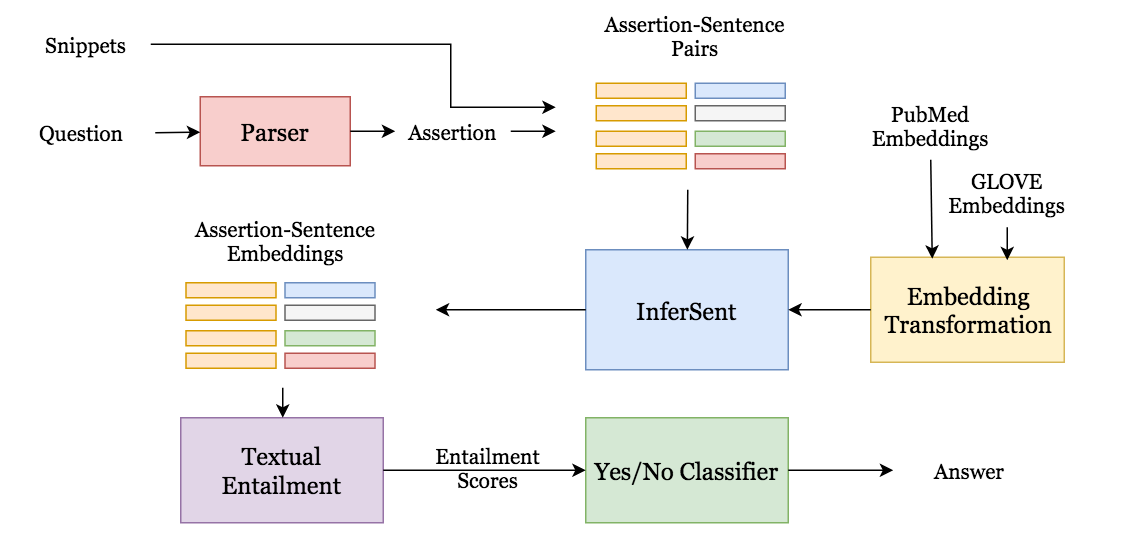
\includegraphics[width=0.95\textwidth]{images/YesNoPipeline.png}
    \caption{The complete system for yes/no answer classification using a question and relevant snippets}
    \label{fig:yesno_pipeline}
\end{figure*}

The end-to-end architecture of our system from the input questions and snippets to the answer is shown Figure \ref{fig:yesno_pipeline}.

\subsubsection{Experimental Details}

For parsing the questions, we used BLLIP (Charniak-Johnson) reranking parser \cite{charniak_new1}
and used the model \texttt{GENIA+PubMed} for biomedical text. For training the textual entailment classifier using \textit{InferSent}'s sentence embeddings, we used Stanford's SNLI \& Multi-NLI dataset \cite{snli} to achieve a test-set accuracy of $84.7 \%$.
%TODO: Specify details for non-linear embedding transformation

\subsubsection{Results}

The performance of the system on yes/no questions on the training set of phase 5b has been tabulated in table \ref{tab:yesno_results}. While the accuracies are better than a random classifier, the task is far from being solved. Nonetheless, the classifier does handle the class bias in the training data and performance similarly on both the categories of answers, which also yields a high F1 score. This is an artifact of the classifier being unsupervised which does not bias it towards skewed distributions in the dataset.

This classifier achieved the best test performance with overall F1 of 65\% on most recent phase (at the time of submission) i.e. phase 4 of BioASQ 6b, and second best test accuracy of 65.6\% on phase 5 of BioASQ 5b (Table \ref{tab:yesno_results}). While we implemented a simple heuristic based answer-classifier, we believe that a supervised classifier using the sentence embeddings as well as fine-tuning of the textual entailment classifier on BioASQ dataset would considerably enhance the overall performance of the system.

\begin{table}[h]
    \centering
    \begin{tabular}{| c | l | l | c | c | c |} \hline
    & \multicolumn{4}{c|}{Accuracy} & \multicolumn{1}{c|}{F1} \\ \hline
    & \multicolumn{2}{c|}{Train} & \multicolumn{2}{c|}{Test} & \multicolumn{1}{c|}{Test} \\ \hline
    & 5b          & 6b &             5b  Phase 5 &          6b Phase 4 & 6b Phase 4 \\ \hline
    Yes         & 0.57 (252/444)  & 0.58 (306/524)     &  -           & -           & 0.7   \\
No          & 0.59 (33/56)    & 0.63 (58/92)       &  -           & -           & 0.6   \\
Overall     & 0.57 (285/500)  & 0.59 (364/616)     &  0.65        & 0.67        & 0.65  \\ \hline
\end{tabular}
    \caption{Class-wise accuracies on yes/no questions for training and test set of BioASQ Phase 5b and 6b}
    \label{tab:yesno_results}
\end{table}

\subsubsection{Error Analysis}

A key challenge in improving the performance of the yes/no system is that it has a lot of modules in sequence, and hence, the attribution of errors in classification becomes difficult. However, we qualitatively analyze the kinds of classification errors depicted in Table \ref{tab:yesno_error_analysis}. 

It can be seen that for a lot of cases for which the model incorrectly incorrectly predicts the answer as \textit{no}, the questions are usually for long. This is most likely because the entailment model fails to perform well on long sentences, since it is trainined on SNLI which mostly consists of short sentences. However, the other types of errors i.e. when the model incorrectly predicts the answer as \text{yes} do no have any clear pattern. 

\begin{table}[h]
    \centering
    \begin{tabular}{|l|c|c|c|} \hline
& Question & Prediction & Answer \\ \hline
\multirow{2}{*}{Correct} & Does metformin interfere thyroxine absorption? & No & No \\  \cline{2-4}
& Is the protein Papilin secreted?  & Yes & Yes \\ \hline
\multirow{6}{*}{Incorrect}
& Is the monoclonal antibody Trastuzumab (Herceptin) & & \\ & of potential use in the treatment of prostate cancer? & No & Yes \\ \cline{2-4}
& Proteomic analyses need prior knowledge of the organism & & \\ 
& complete genome. Is the complete genome of the bacteria & & \\
& of the genus Arthrobacter available? & No & Yes \\ \cline{2-4}
& Is amiodarone a class I anti-arrhythmic drug? & Yes & No \\ \hline
    \end{tabular}
    \caption{Predicted and true answers by the yes/no classifier for some questions in BioASQ dataset 5b}
    \label{tab:yesno_error_analysis}
\end{table}